% !TEX TS-program = pdflatex
% !TEX encoding = UTF-8 Unicode

% This file is a template using the "beamer" package to create slides for a talk or presentation
% - Giving a talk on some subject.
% - The talk is between 15min and 45min long.
% - Style is ornate.

% MODIFIED by Jonathan Kew, 2008-07-06
% The header comments and encoding in this file were modified for inclusion with TeXworks.
% The content is otherwise unchanged from the original distributed with the beamer package.

\documentclass{beamer}
\newtheorem{proposition}{Proposition}


% Copyright 2004 by Till Tantau <tantau@users.sourceforge.net>.
%
% In principle, this file can be redistributed and/or modified under
% the terms of the GNU Public License, version 2.
%
% However, this file is supposed to be a template to be modified
% for your own needs. For this reason, if you use this file as a
% template and not specifically distribute it as part of a another
% package/program, I grant the extra permission to freely copy and
% modify this file as you see fit and even to delete this copyright
% notice. 


\mode<presentation>
{
  \usetheme{Warsaw}
  % or ...

  \setbeamercovered{transparent}
  % or whatever 
}


\usepackage[english]{babel}
% or whatever

\usepackage[utf8]{inputenc}
% or whatever

\usepackage{times}
\usepackage{amsmath}
\usepackage[T1]{fontenc}
% Or whatever. Note that the encoding and the font should match. If T1
% does not look nice, try deleting the line with the fontenc.


\title[Improved Nyström Low Rank Approximation and Error Analysis] % (optional, use only with long paper titles)
{Improved Nyström Low Rank Approximation and Error Analysis}

\author[S. Burova, M. Gjorgjevski] % (optional, use only with lots of authors)
{Sofiya Burova, Martin Gjorgjevski} 
% - Use the \inst{?} command only if the authors have different
%   affiliation.

\institute[ENS Lyon] % (optional, but mostly needed)
{
  ENS Lyon \\
  M2 Advanced Mathematics}
% - Use the \inst command only if there are several affiliations.
% - Keep it simple, no one is interested in your street address.

\date[Short Occasion] % (optional)
{January 2022}

\defbeamertemplate*{footline}{shadow theme}
{%
  \leavevmode%
  \hbox{\begin{beamercolorbox}[wd=.5\paperwidth,ht=2.5ex,dp=1.125ex,leftskip=.3cm plus1fil,rightskip=.3cm]{author in head/foot}%
    \usebeamerfont{author in head/foot}\insertframenumber\,/\,\inserttotalframenumber\hfill\insertshortauthor
  \end{beamercolorbox}%
  \begin{beamercolorbox}[wd=.5\paperwidth,ht=2.5ex,dp=1.125ex,leftskip=.3cm,rightskip=.3cm plus1fil]{title in head/foot}%
    \usebeamerfont{title in head/foot}\insertshorttitle%
  \end{beamercolorbox}}%
  \vskip0pt%
}
\renewcommand{\v}{\vspace{0.5em}}
\subject{Talks}
\date{March 2022}

\begin{document}

\maketitle 

\begin{frame}{Introduction}
 
\begin{itemize}
    \item Nyström method for low rank approximation
    \item Historical motivation and heuristics
    \item Error analysis of a clustered model
    \item New k-means based method 
    \item Empirical test of performance
\end{itemize} 
\end{frame}
\begin{frame}{Nyström Method, what is that?}
Let $K$ be a kernel on a sample set $\mathcal{X}=\{x_i, i\in [n]\}$. Then the Nyström method applied to $K$ using a randomly chosen landmark set $\mathcal{Z}=\{z_i, i \in [m] \}$ approximates the full kernel matrix by 
\begin{block}{Williams and Seeger, 2001}
\begin{equation*}
    K \sim EW^{-1}E^{\prime}
\end{equation*}
where $E$ is an $n\times m$ matrix given by $E_{ij}=k(x_i,z_j) $ and $W$ is an $m\times m$ matrix given by $W_{ij}=k(z_i,z_j) $.
\end{block}

In practice this method promises a lot. 
The most popular sampling scheme is random sampling where a random subset of $m$ points is chosen.
\end{frame}
\begin{frame}{Numerical solutions to integral equations}


\begin{itemize}
    \item Mercer's theorem states that $K(x,y)=\sum_{k=1}^{\infty} \lambda_k \phi_k(x)\phi_k(y)$ 
    with $\phi_k$ orthogonal, $\lambda_k$ nonnegative and decreasing
    \item if $x_j$ are sampled i.i.d. according to $p(x)$, $j=1,2,...,q$, then
    \begin{equation*}
    \int K(x,y)p(y)\phi_k(y)dy\approx \frac{1}{q} \sum_{j=1}^q K(x,x_j)\phi_k(x)
    \end{equation*} 
    by the law of large numbers.
    \item Solve for the eigenvalues of $K^{(q)}=[K(x_i,x_j)]_{1\leq i,j\leq q}$
    \item $\frac{\lambda_k^{(q)}}{q}\approx \lambda_k$, $\lambda_k^{(q)}$ being the k-th largest eigenvalue of $K^{(q)}$\footnote{in fact we have convergence as $q\rightarrow\infty$}
    \item In addition, if $K(x,y)=K(x-y)$ we have
    \begin{equation*}
        \frac{1}{q} \sum_{k=1}^q \lambda_k^{(q)}=\sum_{k=1}^{\infty} \lambda_k
    \end{equation*}
\end{itemize}
\end{frame}
\begin{frame}{Nyström Approximation}
    This approximation is achieved by carrying out an eigendecomposition on a smaller system of size $m<n$:
    
    \begin{itemize}
        \item The method can work well for matrices with rapidly decaying spectra
        \item In practice it is not possible to know which subset of landmark points will have the highest eigenvalue in the spectral decomposition
        \item Error analysis for this method has been limited in the literature
    \end{itemize}
Our objective is to bound the approximation error given by
\begin{equation*}
    \mathcal{E}=\|K-EW^{-1}E^{\prime}\|_F
\end{equation*}
where $\|\cdot\|_F$ denotes the Frobenious norm.



\end{frame}


\begin{frame}{Main result, assumption}
\begin{block}{Assumption A}
Assume that for all $a,b,c,d$,
\begin{equation*}
    (k(a,b)-k(c,d))^2\leq C_{\mathcal{X}}^k (\|a-b\|^2+\|c-d\|^2).
\end{equation*}
where $C_{\mathcal{X}}^k$ is a positive constant depending on $k$ and the sample set $\mathcal{X}$.
\end{block}

\textbf{Remark.} This assumption is valid on many commonly used kernels:
\begin{itemize}
    \item Gaussian kernel, $C_{\mathcal{X}}^k=\frac{1}{2\sigma^2} $
    \item Laplacian kernel, $C_{\mathcal{X}}^k=\frac{1}{\sigma^2} $
    \item Inverse distance kernel, $C_{\mathcal{X}}^k=\frac{1}{\sigma^2 \epsilon^4} $
\end{itemize}
\end{frame}

\begin{frame}{Main result, statement}
Partition $\mathcal{X}$ into $m$ disjoint clusters $S_k, k\in [m]$. \\
\v
Set $c(i) = \textrm{argmin}_{j\in [m]} \|x_i-z_j\| $.
\begin{block}{Theorem}
If the kernel satisfies Assumption A, the error of the Nyström approximation is bounded by
\begin{equation*}
    \mathcal{E} \leq 4T\sqrt{mC_{\mathcal{X}}^k eT}+mC_{\mathcal{X}}^k Te \|W^{-1}\|_F
\end{equation*}
where $T=\max_k|S_k| $ and $e=\sum_{i=1 }^n \|x_i-z_{c(i)}\|^2$ is the total quantization error of coding each sample $x_i \in \mathcal{X}$ with the closest landmark point $z_j \in \mathcal{Z}$.
\end{block}


\end{frame}

\begin{frame}{Main result, sketch of proof}
    The main idea is to decompose the kernel matrix into blocks of size $m \times m$ and bound each \emph{partial approximation error}. This is done via the following sampling process:
    \begin{itemize}
        \item at each time $t$ pick a sample from each cluster and denote the resulting set by $\mathcal{X}_{\mathcal{I}_t}$;
        \item $\mathcal{X} = \cup_{t\in [T]} \mathcal{X}_{\mathcal{I}_t}$;
        \item $K_{\mathcal{I}_i,\mathcal{I}_j}$ and $E_{\mathcal{I}_i,\mathcal{Z}}$ are the $m\times m$ similarity matrices defined resp. on $(\mathcal{X}_{\mathcal{I}_i}, \mathcal{X}_{\mathcal{I}_j} )$ and $(\mathcal{X}_{\mathcal{I}_i}, \mathcal{Z} )$.
        \item $\mathcal{E}_{\mathcal{I}_i,\mathcal{I}_j} = \|K_{\mathcal{I}_i,\mathcal{I}_j} - E_{\mathcal{I}_i,\mathcal{Z}} W^{-1} E^{\prime}_{\mathcal{I}_j,\mathcal{Z}} \|_F $ is the partial approximation error.
    \end{itemize}

    
\end{frame}

\begin{frame}{Main result, sketch of proof}
     Observe that the total error $\mathcal{E} \leq \sum_{i,j=1}^T \mathcal{E}_{\mathcal{I}_i,\mathcal{I}_j}  $. Hence, the following Lemma concludes the proof:
     \begin{block}{Lemma}
     If the kernel satisfies Assumption A, the partial approximation error is bounded by
     \begin{equation*}
     \begin{split}
         \mathcal{E}_{\mathcal{I}_i,\mathcal{I}_j} &\leq \sqrt{2mC_{\mathcal{X}}^k(e_{\mathcal{I}_i}+e_{\mathcal{I}_j})}+\sqrt{mC_{\mathcal{X}}^k e_{\mathcal{I}_i}}\\ &+\sqrt{mC_{\mathcal{X}}^k e_{\mathcal{I}_j}} + m\sqrt{mC_{\mathcal{X}}^k e_{\mathcal{I}_i}} \sqrt{e_{\mathcal{I}_i}e_{\mathcal{I}_j}} \|W^{-1}\|_F
         \end{split}
     \end{equation*}
     where $ e_{\mathcal{I}_i} $ is the quantization error induced by coding each sample in $\mathcal{X}_{\mathcal{I}_i} $ i.e. 
     \begin{equation*}
         e_{\mathcal{I}_i} = \sum_{x_i \in \mathcal{X}_{\mathcal{I}_i}} \|x_i-z_{c(i)}\|^2.
     \end{equation*}
     \end{block}
\end{frame}

\begin{frame}{Conclusion}
For a number of commonly used kernels,in order to minimize the total error of approximation, it suffices to minimize the quantization error
\begin{equation*}
    e=\sum_{i=1 }^n \|x_i-z_{c(i)}\|^2.
\end{equation*}
Naturally, we propose the centers obtained from the $k$-means as the landmark points.
\v
\end{frame}
\begin{frame}{Example}
    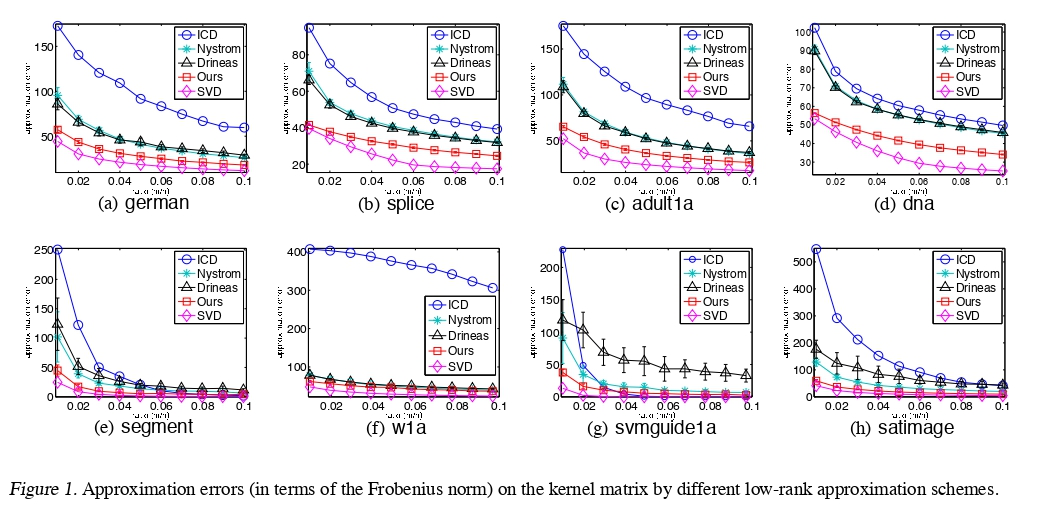
\includegraphics[scale=0.65]{fig1.jpg}
\end{frame}

\end{document}
